\chapter{Text}
\label{ch:text}
At the beginning of the computing era, text was the only medium mediating information between
users and computers. Not only was a textual notation used to denote all kinds of data and objects
via names and numbers (represented by sequences of characters and digits respectively), but
also for the specification of programs (based on the notions of formal language and syntax) and
tasks. Actually, not even the most modern and most sophisticated computing environments have
been able to make falter the dominating role of text substantially. At most, they have introduced
alternative models like graphical user interfaces (GUI) as a graphical replacement for command
lines.

There are many reasons for the popularity of text in general and in connection with computers in
particular. To name but a few: Text containing any arbitrary amount of information can be built
from a small alphabet of widely standardized elements (characters), their building pattern is
extremely simple (lining up elements), and the resulting structure is most elementary (a
sequence). And perhaps most importantly, syntactically structured text can be parsed and
interpreted by a machine.

In computing terminology, sequences of elements are called files and, in particular, sequences of
characters are known as text files. Looking at their binary representation, we find text files
excellently suited to be stored in computer memories and on external media. Remember that
individual characters are usually encoded in one byte each (ASCII-code). We can therefore
identify the binary structure of text files with sequences of bytes, matching perfectly the structure
of any underlying computer storage. We should recall at this point that, with the possible exception
of line-break control characters, rendering information is not part of ordinary text files. For
example, the choices of character style and of paragraph formatting parameters are entirely left to
the rendering interpreter.

Unfortunately, in conventional computing environments, text is merely used for input/output, and
its potential is not nearly exploited optimally. Input texts are typically read from the keyboard under
control of some text editor, interpreted and then discarded. Output text is volatile. Once displayed
on the screen it is no longer available to any other parts of the program. The root of the problem is
easily located: Conventional OSes neither feature an integrated management nor an
abstract programming interface (API) for texts.

Of course, such poor support of text on the level of programming must reflect itself on the user
surface. More often than not, users are forced to retype a certain piece of text instead of simply
copy/pasting it from elsewhere on the screen. Investigations have shown that, in average, up to
80\% of required input text is already displayed somewhere.

Motivated by our positive experience with integrated text in the Cedar system [Teitelman] we
decided to provide a central text management in Oberon at a sufficiently low system level.
However, this is not enough. We actually need an abstract programming interface (API) for text
that is, an abstract data type $Text$, together with a complete set of operations. We shall devote
Section 5.1 to the explanation of this data type. In Section 5.2, we take a closer look at the basic
text management in Oberon, including data structures and algorithms used for the implementation
of type $Text$.

Text frames are a special class of display frames. They appear typically (but not necessarily) as
frames within a menu viewer (see Section 4.4.2). Their role is double-faced: a) Rendering text on
the display screen and b) interpreting interactive editing commands. The details will be discussed
in Section 5.3.

With the aim of exploiting the power of modern bitmap-displays and also of reusing the results of
earlier projects in the field of digital font design, we decided in favor of supporting “rich texts” in
Oberon, including graphical attributes and in particular font specification. In Section 5.4 we shall
explain the font machinery, starting from an abstract level and proceeding down to the level of
raster data.

\section{Text as an abstract data type}
The concept of abstraction is arguably the most important achievement of programming language
development. It provides a powerful tool to create simplified views of complicated things and
connections. Two prominent examples of program abstractions are definitions (interfaces) and
abstract data types, embodying simplified views on a certain piece of program and on a certain kind
of data respectively.

We shall now give a precise definition of the notion of text in Oberon by presenting it as an abstract
data type. It is important not to confuse this type with the far less powerful type String as it is often
supported by advanced programming languages. In this Section we carefully avoid revealing any
implementation aspects of the abstract type Text. Our viewpoint is that of an application program
operating on text abstractly or using it as a medium of communication.

Nevertheless, let us first use a symbolic looking glass to get a refined understanding of the concept
of character in the context of rich texts. We know that each character represents a textual element
of information. If displayed, it also refers to some specific graphical pattern, often called glyph. In
Oberon, we do justice to both aspects by thinking of the ASCII-code as an index into a font that is
into a set of glyphs of the same style. Representing characters as pairs (font, ref), where font
designates a font and ref the character's ASCII-code and adding two more attributes color and
vertical offset, we get to a quadruple representation (font, ref, col, voff) of characters. The
components font, color, and vertical offset together are often referred to as looks. With that, we can
now define a (rich) text as a sequence of characters with looks. We shall treat the topic of fonts and
glyphs thoroughly in Section 5.4.

For the moment, however, let us continue our discussion of the abstract data type Text. Formally,
we define it as
\begin{verbatim}
  Text = POINTER TO TextDesc;
  TextDesc = RECORD
    len: INT;
    notify: Notifier
  END;
\end{verbatim}
There is only one state variable and one method. The variable len represents the current length of
the described text (i.e. the number of characters in the sequence). The procedure variable notify is
included as a method (occasionally called after-method) to notify interested clients of state
changes.

By definition, each abstract data type comes with a complete set of operations. In the case of Text,
three different groups corresponding to three different topics need to be considered, loading (from
file), storing (to file), editing, and accessing (reading and writing) respectively.

\subsection{Loading and Storing Text}
Let us start with the file group. We first introduce a pair of mutually inverse operations called
internalize and externalize. Their meaning is "load from file and build up an internal data structure"
and "serialize the internal data structure and store it on file" respectively. There are three
corresponding procedures:
\begin{verbatim}
  PROC Open (T: Text; name: ARRAY OF CHAR);
  PROC Load (T: Text; f: Files.File;
                  pos: INT; VAR len: INT);
  PROC Store (T: Text; f: Files.File;
                  pos: INT; VAR len: INT);
\end{verbatim}
Logical entities like texts are stored in Oberon on external media in the form of sections. A section
is addressed by a pair (file, pos) consisting of a file descriptor and a starting position. In general, the
structure of sections obeys the following syntax:
\begin{verbatim}
  section = identification type length contents.
\end{verbatim}

Procedure Open internalizes a named text file (consisting of a single text section), procedure Load
internalizes an arbitrary text section starting at (f, pos), and procedure Store externalizes a text
section to (f, pos). The parameter T designates the internalized text. len returns the length of the
section. Note that in case of Load the identification of the section must have been read and
consumed before the loader is called.

\subsection{Editing Text}
Our next group of operations supports text editing. It comprises four procedures:
\begin{verbatim}
  PROC Delete (T: Text; beg, end: INT);
  PROC Insert (T: Text; pos:INT; B:Buffer);
  PROC Append (T: Text; B: Buffer);
  PROC ChangeLooks (T: Text; beg, end: INT;
     sel: SET; fnt: Fonts.Font; col, voff: INT);
\end{verbatim}
Again, we should first explain the types of parameters. Procedures Delete and ChangeLooks each
take a stretch of text as an argument which, by definition, is an interval [beg, end) within the given
text. In the parameter lists of Insert and Append we recognize a new data type Buffer.
Buffers are a facility to hold anonymous sequences of characters. Type Buffer presents itself again
as an abstract data type:
\begin{verbatim}
  Buffer = POINTER TO BufDesc;
  BufDesc = RECORD len: INT END;
\end{verbatim}
$len$ specifies the current length of the buffered sequence. The following procedures represent the intrinsic operations on buffers:
\begin{verbatim}
  PROC OpenBuf (B: Buffer);
  PROC Copy (SB, DB: Buffer);
  PROC Save (T:Text; beg,end:INT; B:Buffer);
\end{verbatim}

Their function is in turn opening a given buffer B, copying a buffer SB to DB, saving a stretch [beg,
end) of text in a given buffer, and recalling the most recently deleted stretch of text and putting it
into buffer B.

Buffer is used as an auxiliary data type in editing procedures. Procedure Delete deletes the given
stretch [beg, end) within text T, Insert inserts the buffer's contents at position pos within text T, and
Append(T, B) is a shorthand form for Insert(T, T.len, B). Note that, as a side-effect of Insert and
Append, the buffer involved is emptied. Finally, procedure ChangeLooks allows to change selected
looks within the given stretch [beg, end) of text T. sel is a mask selecting a subset of the set of
looks { font, color, vertical offset }.

It is time now to come back to the notifier concept. Recapitulate that notify is an “after-method”. It
must be installed by the client when opening the text and is called at the end of every editing
operation. Its signature is
\begin{verbatim}
  Notifier = PROC(T:Text; op,beg,end:INT);
\end{verbatim}
The parameters $op$, $beg$, and $end$ report about the operation ($op$) that calls the notifier and on the
affected stretch $[beg, end)$ of the text. There are three different possible variants of $op$
corresponding to the three different editing operations: $op =$ delete, insert, replace correspond to
procedures $Delete$, $Insert$(, $Append$), and $ChangeLooks$ respectively.

By far the most important application of the notifier is updating the display, i.e. adjusting all affected
views of the text that are currently displayed to the new state of the text (the model). We shall come
back to this important matter when discussing text frames in Section 5.3.

In concluding this Section it is worth noting that the groups of operations just discussed have been
designed to be equally useful for interactive text editors as for programmed text generators/manipulators.

\subsection{Accessing Text}
Let us now turn to the third and last group of operations on texts: Accessing that is reading and
writing. According to the principle of separation of concerns, one of our guiding principles, the
access mechanism operates on extra aggregates called readers and writers rather than on texts
themselves.

Readers are used to read texts sequentially. Their type is declared as
\begin{verbatim}
  Reader = RECORD
    eot: BOOL; (*end of text*)
    fnt: Fonts.Font;
    col, voff: INT
  END;
\end{verbatim}

A reader must first be opened at the desired position in the text before it can then be moved
forward incrementally by reading character-by-character. Its state variables indicate end-of-text and
expose the looks of the character last read.
The corresponding operators are
\begin{verbatim}
  PROC OpenReader (VAR R: Reader; T: Text;
                                     pos: INT);
  PROC Read (VAR R: Reader;  VAR ch: CHAR);
\end{verbatim}

Procedure $OpenReader$ sets up a reader $R$ at position $pos$ in text $T$. Procedure $Read$ returns the
character at the current position of $R$ and makes $R$ move to the next position.
The current position of reader $R$ is returned by a call to the function $Pos$:
\begin{verbatim}
  PROC Pos (VAR R: Reader): INT;
\end{verbatim}

In Chapter 3 we learned that commands plus parameter lists are often embedded in ordinary texts.
When interpreting such commands, the underlying text appears as a sequence of tokens like name,
number, special symbol etc. much rather than as a sequence of characters. Therefore, we have
adopted the well-known concepts of syntax and scanning from the discipline of compiler
construction, including functional support. The Oberon scanner recognizes tokens of some
universal classes. They are name, string, integer, real, longreal, and special character.
The exact syntax of universal Oberon tokens is:
\begin{verbatim}
token = name | string | integer | real | spexchar.
name = ident { "." ident }.ident
     = letter { letter | digit }.
string = """ { char } """.
integer = ["+"|"-"] number.
real = ["+"|"-"] number "." number ["E" ["+"|"-"] number].
number = digit { digit }.
spexchar = any character except letters, digits,
                space, tab, and carriage-return.
\end{verbatim}
Type Scanner is defined correspondingly as
\begin{verbatim}
  Scanner = RECORD (Reader)
    nextCh: CHAR;
    line: INT;
    class: INT;
    i: INT;
    x: REAL;
    c: CHAR;
    len: INT;
    s: ARRAY 32 OF CHAR
  END;
\end{verbatim}

This type is actually a variant record type with class as discriminating tag. Depending on its class
the value of the current token is stored in one of the fields i, x, c, or s. len gives the length of s,
nextCh typically exposes the character terminating the current token, and line counts the number of
lines scanned.

The operations on scanners are
\begin{verbatim}
  PROC OpenScanner (VAR S: Scanner; T: Text;
                                     pos: INT);
  PROC Scan (VAR S: Scanner);
\end{verbatim}

They correspond exactly to their counterparts OpenReader and Read respectively.
Writers are dual to readers. They serve the purpose of creating and extending texts. However,
again, they do not operate on texts directly. Rather, they act as self-contained aggregates,
continuously consuming and buffering textual data.

The formal declaration of type Writer resembles that of type Reader:
\begin{verbatim}
  Writer = RECORD
    buf: Buffer;
    fnt: Fonts.Font;
    col, voff: INT
  END;
\end{verbatim}

$buf$ is an internal buffer containing the consumed data. $fnt$, $col$, and $voff$ specify the current looks for
the next character consumed by this writer.

The following procedures constitute the Writer API:
\begin{verbatim}
  PROC OpenWriter (VAR W: Writer);
  PROC SetFont (VAR W: Writer; fnt:Fonts.Font);
  PROC SetColor (VAR W: Writer; col: INT);
  PROC SetOffset (VAR W: Writer; voff:INT);
\end{verbatim}

Procedure OpenWriter opens a new writer with an empty buffer. Procedures SetFont, SetColor, and
SetOffset set the respective current look. For example, SetFont(W, fnt) is equivalent with W.fnt :=
fnt. These procedures are included because fnt, col, and voff are read-only for clients.

The question may arise how data is produced and transferred to writers. The answer is a set of
writer procedures, each of them handling an individual data type:
\begin{verbatim}
PROC Write (VAR W: Writer; ch: CHAR);
PROC WriteLn (VAR W: Writer);
PROC WriteString (VAR W:Writer; s:ARRAY OF CHAR);
PROC WriteInt (VAR W: Writer; x, n: INT);
PROC WriteHex (VAR W: Writer; x: INT);
PROC WriteReal (VAR W:Writer; x:REAL; n:INT);
PROC WriteRealFix (VAR W: Writer; x: REAL;
                                    n, k: INT);
PROC WriteClock(VAR W: Writer; d: INT);
\end{verbatim}

The following is schematic fragment of a client program that creates textual output:
\begin{verbatim}
  open writer; set desired font;
  REPEAT
    process;
    write result to writer;
    append writer buffer to output text
  UNTIL ended
\end{verbatim}
Of course, writers can be reused. For example, a single global writer is typically shared by all of the
procedures within a module. In this case, the writer needs to be opened just once at module loading
time.

Typically, however, accessing aggregates are of a transient nature and are bound to a certain
activity, which manifests itself in their allocation on the stack without any possibility of referencing
them from the outside of the activity, in contrast to the underlying texts that are allocated on the
system heap and have a much longer life time.

Let us summarize: Text in Oberon is a powerful abstract data type with intrinsic operations from
three areas: Loading/storing, editing, and accessing (reading/writing). The latter two areas on their
part introduce further abstract types called Buffer, Reader, Scanner, and Writer. In combination
they guarantee a clean separation of very different concerns. The benefits of such a rigorous
decoupling are numerous. For example, it makes it possible to freely choose (and vary) the
granularity at which a text and its views are updated. Finally, an after-method is used to allow
context-dependent post-processing of editing operations. It is used primarily for preserving
consistency between text models and their views.

\section{Text Management}
The art and challenge of modularization lie in finding an effective decomposition of a topic into
modules with relatively thin interfaces or, in other words, into modules with a great potential for
information hiding. Text systems provide a welcome opportunity of an exercise. A closer analysis
immediately leads to the following separate concerns corresponding to the components Model,
View and Controller of the MVC scheme: Text management, text rendering, and text editing. If we
combine View and Controller and add an auxiliary font handling module Fonts, we arrive at the
following three-module import hierarchy:
\begin{table}[h!]
	\begin{tabular}{l l l}
		Module     &Object type &Service \\\hline
		TextFrames &Frame       &Text rendering and editing\\
		Texts      &Text        &Text management \\
		Fonts      &Font        &Font management
	\end{tabular}
\end{table}

Note that, in contrast to the display-subsystem, the associated object types are not connected hierarchically here.

Separate Sections 5.3 and 5.4 will be devoted to modules TextFrames and Fonts respectively. In
the current Section we focus on module Texts. Regarding it as a model of the abstract data type
Text presented in the previous Section, its definition is congruent with the specification of the
abstract data type itself, and we need not repeat it here.

The main topics of this Section are internal representation and file representation of texts. We first
emphasize that the internal representation of a text is a completely private matter of module Texts
that is encapsulated and hidden from clients. In particular, the representation could be changed at
any time without invalidating any single client. In principle, the same is true for the file
representation. However, stability is of paramount importance here because files serve the
additional purposes of backing up text on external media and of porting text to other environments.
Our choice of an internal representation of text was determined by a catalogue of requirements and
desired properties. The wish list looks like this:
\begin{enumerate}
	\item lean data structure
	\item closed under editing operations
	\item efficient editing operations
	\item efficient sequential reading
	\item efficient direct positioning
	\item super efficient internalizing
	\item preserving file representations
\end{enumerate}
With the exception of 5., we found these requirements met perfectly by an adequately generalized
variant of the piece list technique that was originally used for Xerox PARC's Bravo text editor and
also for ETH's former document editors Dyna and Lara [Gutknecht]. The original piece list is able to
describe a vanilla text without looks. It is based on two principles:
\begin{enumerate}
	\item A text is regarded as a sequence of pieces, where a piece is a section of a text file consisting of
a sequence of contiguous characters.
	\item Every piece is represented by a descriptor (f, pos, len), where the components designate a file,
a starting position, and a length respectively. The whole text is represented as a list of piece
descriptors (in short: piece list). The editing operations operate on the piece list rather than on the
pieces themselves.
\end{enumerate}

If the entire life of our planet were represented by one twenty-four-hour day,
intelligent life appeared within the last few seconds
\begin{figure}
	\label{fig:chain}
	\centering
	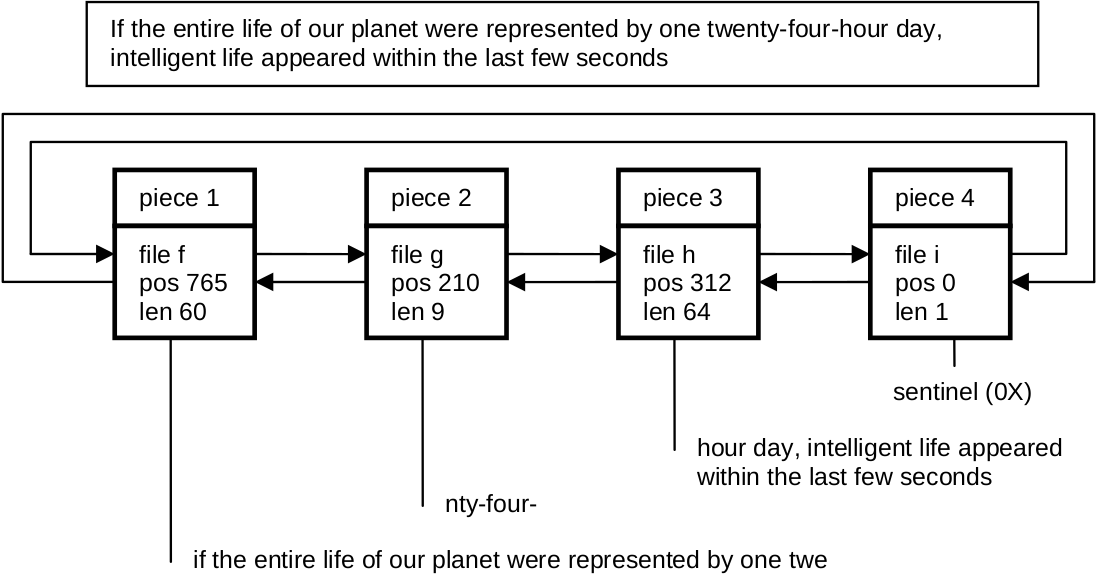
\includegraphics[width=\textwidth]{i/d}
	\caption{Piece chain representing a text}
\end{figure}

Fig \ref{fig:chain} shows a typical piece list representing (the current state of) a text. Investigating the
effects of the basic editing operations delete and insert on the piece list, we end up with these
algorithms:
\begin{verbatim}
delete stretch [beg, end) of text = BEGIN
  split pieces at beg and at end;
  remove p-descriptors from beg to end from the chain
END

insert stretch of text at pos = BEGIN
  split piece at pos;
  insert p-descriptors representing the stretch at pos
END
\end{verbatim}
Of course, splitting is superfluous if the desired splitting point happens to coincide with the
beginning of a piece. Fig \ref{fig:chain-after-insert} and \ref{fig:chain-generalized} show the resulting piece list after a delete and an insert operation respectively.
If the entire life of our planet were represented by one day, intelligent life
appeared within the last few seconds
\begin{figure}
	\label{fig:chain-after-delete}
	\centering
	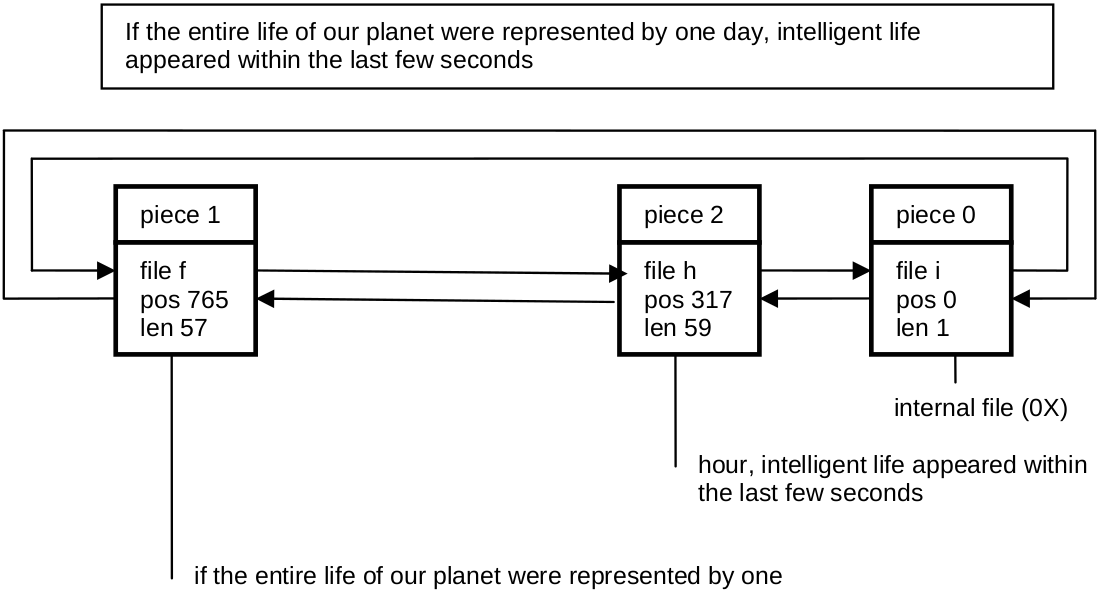
\includegraphics[width=\textwidth]{i/e}
	\caption{Piece chain after delete operation}
\end{figure}

If the entire life of our plane, from its origin to the present moment, were
represented by one day, intelligent life appeared within the last few seconds
\begin{figure}
	\label{fig:chain-after-insert}
	\centering
	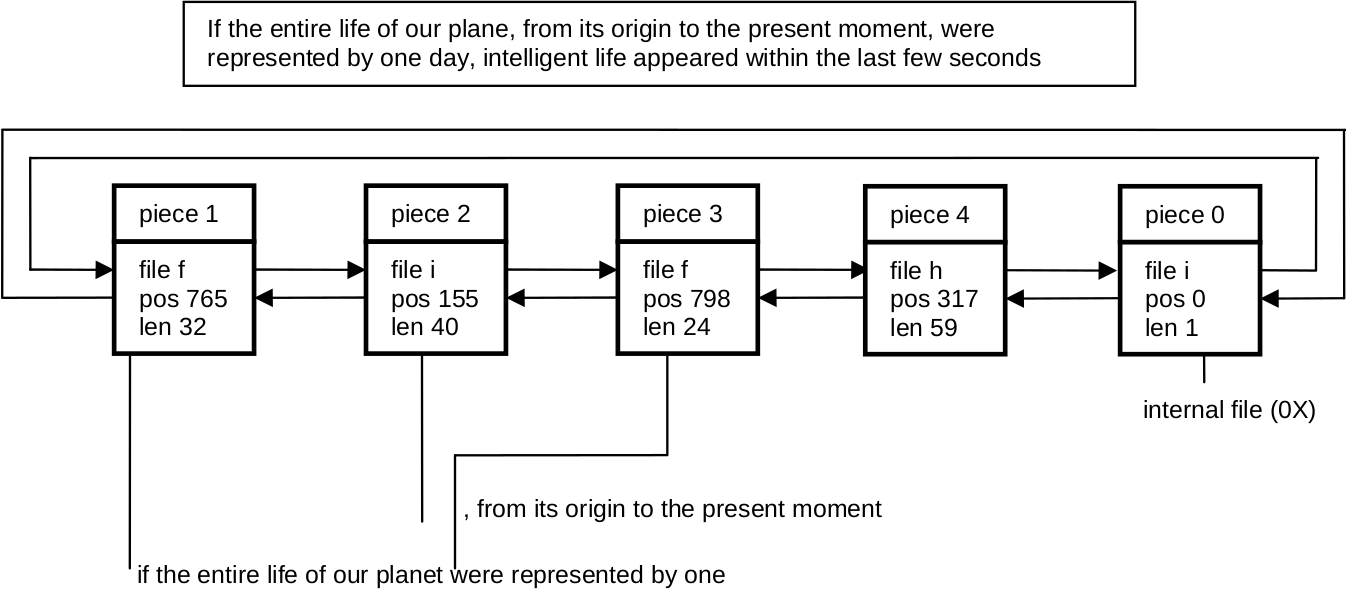
\includegraphics[width=\textwidth]{i/f}
	\caption{Piece chain after insert operation}
\end{figure}

Checking our wish list of above we immediately recognize the requirements 1.), 2.), and 3.) as met.
Requirement 4.) is also met under the assumption of an efficient mechanism for direct positioning in
files. Requirement 6.) can be checked off because the piece list initially consists of a single piece
spanning the entire text file. Finally, requirement 7.) is met simply because the operations do not
affect file representations at all.

In Oberon we adapted the piece list technique to texts with looks ("rich texts"). Formally, we first
define a run as a stretch of text whose characters show identical looks. Now, we require the piece
list to subordinate itself to the run structure. This obviously means that every piece needs to be
contained within a single run. Figure 5.4 visualizes such a compliant piece list representing a text
with varying looks. There are only two new aspects compared to the original version of the piece list
discussed above: An additional operation to change looks and the initial state of the piece chain.
\begin{verbatim}
change looks in a stretch [beg, end) of text = BEGIN
split pieces at beg and at end;
change looks in piece descriptors from beg to end in the chain
END
\end{verbatim}
This shows that requirements 2.) and 3.) in the wish list are still satisfied.
I have trained that man, says the laboratory rat, so that every time I press this lever
he gives me food
\begin{figure}
	\label{fig:chain-generalized}
	\centering
	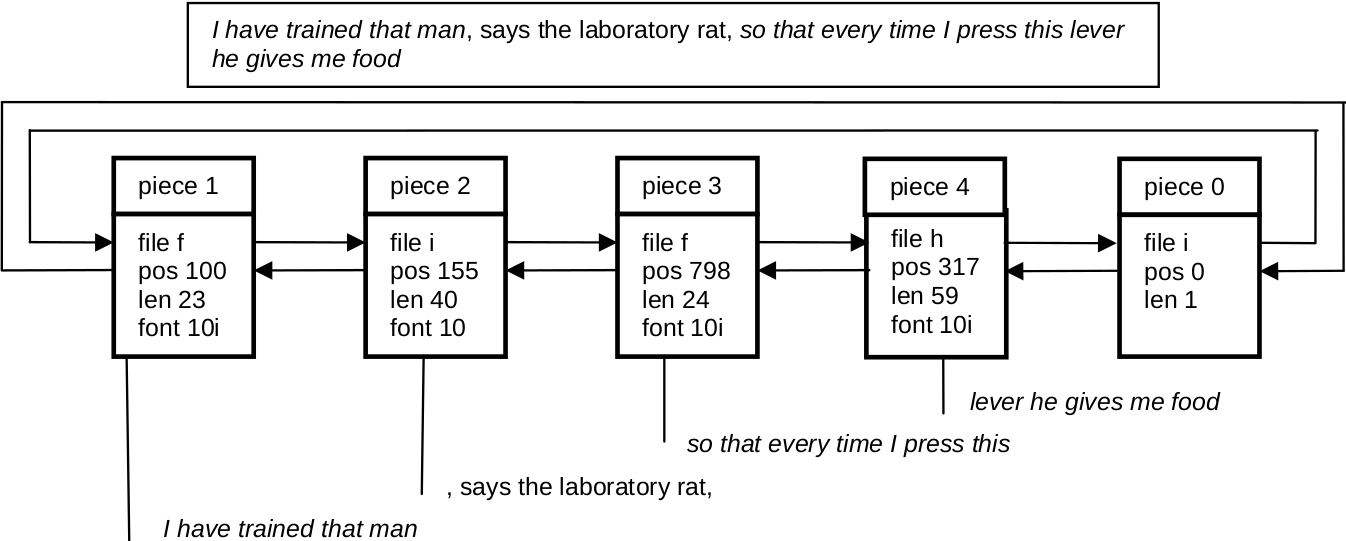
\includegraphics[width=\textwidth]{i/g}
	\caption{Generalized piece chain representing a text with looks}
\end{figure}

Initially, the pieces are identical with runs, and the number of elements in the piece list is equal to
the number of runs. Because this number is typically small in comparison with the total number of
characters in a text requirement 6.) is still met.

We conclude that the new aspects do not invalidate the positive rating given above to the piece
technique with regard to requirements 1.), 2.), 3.), 4.), 6.), and 7.) in our wish list. However, the
requirement of efficient direct positioning remains. The problem is the necessity to scan through the
piece list sequentially in order to locate the piece that contains the desired position. We investigated
different solutions of this efficiency problem. They are based on different data structures connecting
the piece descriptors, among them a piece tree and a variant of the piece list featuring an additional
long-distance link like in a skip-list.

Eventually, we decided in favor of a simpler solution that we can easily justify by pointing out that
the typical editing scenario is zooming into a local region of text, i.e. positioning at an arbitrary
location once and subsequently positioning at locations in its immediate neighborhood many times.
Therefore, an appropriate solution is caching the most recently calculated values (pos, piece) of the
translation map. Of course, this does not solve the problem of cache misses. Notice, however, that
this problem is acute only in the case of extremely long piece lists that do not occur in ordinary texts
and editing sessions.

We shall now illustrate the piece technique in detail at the example of two important but basic
operations: Insert and read. Let us start with an overview of the data types involved. Apart from
some auxiliary private variables marked with an arrow, the types Text, Buffer, and Reader are
already familiar to us from the previous Section. Type Piece is completely private and hidden from
the clients.
\begin{verbatim}
Text = POINTER TO TextDesc;
Notifier = PROC (T: Text; op, beg, end: INT);

TextDesc = RECORD
len: INT;
notify: Notifier;
--> trailer: Piece;
--> org: INT;
--> pce: Piece
END;

Buffer = POINTER TO BufDesc;
BufDesc = RECORD
len: INT;
--> header, last: Piece
END;

Reader = RECORD
eot: BOOL;
fnt: Fonts.Font;
col, voff: INT;
--> ref: Piece;
--> org, off: INT;
rider: Files.Rider
END;

--> Piece = POINTER TO PieceDesc;
--> PieceDesc = RECORD
f: Files.File;
off, len: INT;
fnt: Fonts.Font;
col, voff: INT;
prev, next: Piece
END;
\end{verbatim}

As depicted in Figure 5.1, the piece list is implemented as a doubly linked list with a sentinel piece
closing it to a ring. The field trailer in type TextDesc points to the sentinel piece. Fields org and pce
implement a translation cache consisting of merely one entry (org, pce). It links a position org with a
piece pce. The fields header and last in type Buffer refer to the implementation of buffers as piece
lists. They point to the first and last piece descriptors respectively. Finally, the fields ref, org, and off
in type Reader memorize the current piece, its origin, and the current offset within this piece.
The fields f, off, and len in type Piece specify the underlying file, starting position in the file, and
length of the piece. fnt, col, and voff are its looks. Finally prev and next are pointers to the previous
piece and to the next piece in the list respectively.

FindPiece and SplitPiece are auxiliary procedures that are used by almost all piece-oriented
operations.
\begin{verbatim}
PROC FindPiece (T: Text; pos: INT; VAR org: INT; VAR p: Piece);
VAR p: Piece; porg: INT;
BEGIN p := T.pce; porg := T.org;
1) IF pos >= porg THEN
WHILE pos >= porg + p.len DO INC(porg, p.len); p := p.next END
2) ELSE p := p.prev; DEC(porg, p.len);
WHILE p < porg DO p := p.prev; DEC(porg, p.len) END
END;
3) T.pce := p; R.org := porg; (*update cache*)
pce := p; org := porg
END FindPiece;
\end{verbatim}

Explanations (referring to the line numbers in the above code excerpt)
1) search to the right (next)
2) search to the left (prev)
3) update cache if more than 50 pieces traversed
\begin{verbatim}
1) PROC SplitPiece (p: Piece; off: INT; VAR pr: Piece);
VAR q: Piece;
BEGIN
2) IF off > 0 THEN NEW(q);
q.fnt := p.fnt; q.col := p.col; q.voff := p.voff;
q.len := p.len - off;
q.f := p.f; q.off := p.off + off;
p.len := off;
q.next := p.next; p.next := q;
q.prev := p; q.next.prev := q;
pr := q
ELSE pr := p
END
END SplitPiece;

3)
4)
\end{verbatim}

Explanations:
1)
2)
3)
4)

return right part piece pr after split
generate new piece only if remaining length > 0
insert new piece in forward chain
insert new piece in backward chain

Procedure Insert handles text insertion. It operates on a buffer that contains the stretch of text to be inserted:
\begin{verbatim}
PROC Insert (T: Text; pos: INT; B: Buffer);
VAR pl, pr, p, qb, qe: Piece; org, end: INT;
BEGIN
1) FindPiece(T, pos, org, p); SplitPiece(p, pos - org, pr);
2) IF T.org >= org THEN
T.org := org - p.prev.len; T.pce := p.prev
END;
pl := pr.prev; qb := B.header.next;
3) IF (qb # NIL) & (qb.f = pl.f) & (qb.off = pl.off + pl.len)
& (qb.fnt = pl.fnt) & (qb.col = pl.col) & (qb.voff = pl.voff) THEN
pl.len := pl.len + qb.len; qb := qb.next
END;
IF qb # NIL THEN qe := B.last;
4)
qb.prev := pl; pl.next := qb; qe.next := pr; pr.prev := qe
END;
5) T.len := T.len + B.len; end := pos + B.len;
6) B.last := B.header; B.last.next := NIL; B.len := 0;
7) T.notify(T, insert, pos, end)
END Insert;
\end{verbatim}

Explanations:
1)
2)
3)
4)
5)
6)
7)

split piece to isolate point of insertion
adjust cache if necessary
merge pieces if possible
insert buffer
update text length
empty buffer
notify

Procedure Read implements sequential reading of characters in texts. It operates on a text reader:
\begin{verbatim}
PROC Read (VAR R: Reader; VAR ch: CHAR);
BEGIN
1) Files.Read(R.rider, ch); R.fnt := R.ref.fnt; R.col := R.ref.col; R.voff := R.ref.voff;
INC(R.off);
2) IF R.off = R.ref.len THEN
3) IF R.ref.f = WFile THEN R.eot := TRUE END;
R.org := R.org + R.off; R.off := 0;
4) R.ref := R.ref.next; R.org := R.org + R.off; R.off := 0;
5) Files.Set(R.rider, R.ref.f, R.ref.off)
END
END Read;
\end{verbatim}

Explanations:
1)
2)
3)
4)
5)

read character from file and update looks in reader
if piece boundary reached
check if sentinel piece reached
move reader to next piece
position file rider

Procedure Read is typically used as a primitive by text scanners and in particular by the built-in
scanner Scan for the recognition of universal tokens, as they were defined in the previous section.
Scanning is a rather complex operation that, for example, includes the conversion of a sequence of
digits into an internal floating-point representation and vice-versa. Scanning a real number involves
recognizing m and d, and computing x = m*10d. This is done using procedure Ten(d) computing 10d
by repeated multiplication maintaining the invariant t * pn = 10n0, where n0 is the initial value of n.
\begin{verbatim}
PROC Ten(n: INT): REAL;
VAR t, p: REAL;
BEGIN t := 1.0; p := 10.0;
WHILE n > 0 DO
IF ODD(n) THEN t := p * t END ;
p := p*p; n := n DIV 2
END ;
RETURN t
END Ten;
\end{verbatim}

Writing a real number in decimal form is more complicated. It involves the computation of m and d
from x = n*2e so that x = m*10d with $1.0 \leq m < 10.0$. First, e is obtained with the standard function
UNPK(x, e), then d is computed (from the relationship 10k = 2k*log(10)) as d = e/log2(10). In order to
avoid a real division for obtaining d, we use the approximation 1.0 / log2(10) = 77 DIV 256, and then
compute x := x / Ten(e) or x := x * Ten(-e). Further details are to be taken from the listings of
WriteReal and WriteRealFix.

In spite of its apparent simplicity the piece list technique interoperates with other system
components in quite a subtle way. For example, after a while of editing, there are typically
numerous cross references between the documents involved. In other words, pieces of one
document may point to foreign files that is to files that were originally associated with other
documents. As a consequence, the FS must either employ some smart garbage collection
algorithm or not recycle file pages at all, even if a new version of a file of the same name has been
created in the meantime.

A problem of another kind, again affecting the FS, arises if, say, a single text line is
composed of several small pieces. Then, reading this line sequentially may necessitate several
jumps to different positions in different files at a high pace. Depending on the quality of the file
buffering mechanism, this may lead to significantly hesitant mouse tracking.

And finally, typed characters that are supposed to be inserted into a text need to be stored on the
so-called keyboard file. For this (continuously growing) file, several readers and one writer must be
allowed to coexist concurrently.

As a consequence, the following qualities of the underlying FS are mandatory for the piece
technique to work properly:
\begin{enumerate}
	\item Once a file page is allocated it must not be reused (until system restart).
	\item A versatile file buffering mechanism supporting multiple buffers per file is required.
	\item Files must be allowed to be open in read mode and in write mode simultaneously.
\end{enumerate}
The format of text sections in files obeys a set of syntactical rules (productions) that can easily be
specified in EBNF-notation:
\begin{verbatim}
TextSection = ident header {char}.
header = type offset run {run} null length.
run = font [name] color offset length.
\end{verbatim}

In the TextSection production ident is an identifier for text blocks. In the header production type is a
type-discriminator, offset is the offset to the character part, run is a run-descriptor, null is a nullcharacter, and length is the length of the character sequence. In the run production font, color, and
offset are specifications of looks, and length is the run-length. In order to save space, font names
are coded as ordinal numbers within a text section. If and only if a font appears for the first time in a
text block it is followed by the actual font name.

Let us conclude this Section with two side-remarks and a summary.
Remarks:
For compatibility reasons, plain ASCII-files are accepted as text files as well. They are mapped
to texts consisting of a single run with standard looks.

Internalizing a text section from a file is extremely efficient because it is obviously sufficient to
read the header and translate it into the initial state of the piece list.

Summary: The mechanism used for the implementation of the abstract data type Text is completely
hidden from clients. It is a generalized version of the original piece list technique, adapted to texts
with looks. The piece list technique in turn is based on the principle of indirection: Operations
operate on descriptors of texts rather than on texts themselves. The benefits are efficiency and
non-destructive operations. However, the technique works properly only in combination with an
efficient (and reliable) garbage collector and a suitable FS.

\section{Text Frames}
The tasks of text frames are text rendering and user interaction. A text frame represents a text view
and a controller in the form of an interactive text editor. Technically, text frames are a subclass of
display frames and, as such, are objects with an open message interface of the kind explained in
Chapter 4.

The geometric layout of text frames is determined by two areas: A rectangle of contents and a
vertical scroll-bar along the left borderline. The type of text frames is a direct extension of type
Display.Frame:
\begin{verbatim}
Frame = POINTER TO FrameDesc;
FrameDesc = RECORD (Display.FrameDesc)
text: Texts.Text;
org, col, lsp: INT;
left, right, top, bot: INT;
markH, time: INT;
hasCar, hasSel, hasMark: BOOL;
carloc: Location;
selbeg, selend: Location
END;
\end{verbatim}

Fields text and org specify the text part to be displayed, the former referring to the underlying text
and the latter designating the starting position of the displayed part. Fields col and lsp are rendering
parameters. They specify the frame's background color and the line spacing. Fields left, right, top,
and bot are margins. They determine the rectangle of contents. mark indicates whether there is a
position marker, which is a small horizontal bar indicating the position of the displayed part relative
to the whole text. markH represents its location within the text frame.

Caret and selection are two important features associated with a text frame. The caret indicates a
focus, and it serves as an implicit "point of insertion" for placing consumed characters (for example
from the keyboard). The selection is a stretch of displayed text. Additionally it serves as a
parameter for various operations and commands, among them delete and change looks. The state
and location of the caret is given by the variables car and carloc respectively. Analogously, the
state of the selection and its begin and end are reflected by the fields sel, selbeg, and selend in the
frame descriptor. Field time is a time stamp on the current selection.

In principle, caret and selection could be regarded as ingredients of the underlying text (the model)
equally well. However, we deliberately decided to associate these features with frames (views) in
order to get increased flexibility. For example, two different selections in adjacent viewers
displaying the same text are normally interpreted as one extensive selection across their span.
The auxiliary type Location summarizes information about a location in a text frame. Its definition is:
\begin{verbatim}
Location = RECORD
org, pos, dx, x, y: INT
END;
\end{verbatim}

x, y specify the envisioned location relative to the text frame's origin, and dx is the width of the
character at this location. pos is the corresponding position in the text and org is the origin position
of the corresponding text line.

The following is a simplified version of the message handler employed by text frames. It fully
determines the behavior and capabilities of text frames.
\begin{verbatim}

1)
2)

3)
4)
5)
7)
8)
9)

PROC Handle* (F: Display.Frame; VAR M: Display.FrameMsg);
VAR F1: Frame; buf: Texts.Buffer;
BEGIN
CASE M OF
Oberon.InputMsg:
IF M.id = Oberon.track THEN Edit(F(Frame), M.X, M.Y, M.keys)
ELSIF M.id = Oberon.consume THEN
IF F(Frame).hasCar THEN Write(F(Frame), M.ch, M.fnt, M.col, M.voff) END
END |
Oberon.ControlMsg:
IF M.id = Oberon.defocus THEN Defocus(F(Frame))
ELSIF M.id = Oberon.neutralize THEN Neutralize(F(Frame))
END |
Oberon.SelectionMsg:
GetSelection(F(Frame), M.text, M.beg, M.end, M.time) |
Oberon.CopyMsg: Copy(F(Frame), F1); M.F := F1 |
MenuViewers.ModifyMsg: Modify(F(Frame), M.id, M.dY, M.Y, M.H) |
CopyOverMsg: CopyOver(F(Frame), M.text, M.beg, M.end) |
UpdateMsg: IF F(Frame).text = M.text THEN Update(F(Frame), M) END
END
END Handle;
\end{verbatim}

Explanations:
1)
2)
3)
4)
5)
6)
7)
8)
9)

Mouse tracking message: Call built-in editor immediately
Consume message: In case of valid caret insert character
Defocus message: Remove caret
Neutralize message: Remove caret and selection
Selection message: Return current selection with time stamp
Copyover message: Copy given stretch of text to caret
Copy message: Create a copy (clone)
Modify message: Translate and change size
Update message: If text was changed then update display

We recognize again our categories of universal messages introduced in Chapter 4, Table 4.6:
Messages in lines 1) and 2) report about user interactions. Messages in 3), 4), 5), 6), and 7) specify
generic operations. Messages in 8) require a change of location or size. Messages of the latter kind
arrive from the ancestor menu viewer via delegation. They are generated by the interaction handler
and preprocessed by the original viewer message handler. Finally, messages in line 9) report about
changes of contents.

The text frame handler is encapsulated in a module called TextFrames. This module exports the
above introduced types Frame (text frame) and Location, as well as the procedure Handle.
Furthermore, it exports type UpdateMsg to report on changes made to a displayable text.
\begin{verbatim}
UpdateMsg = RECORD (Display.FrameMsg)
id: INT;
text: Texts.Text;
beg, end: INT
END;
\end{verbatim}

Field id names one of the operators replace, insert, or delete. The remaining fields text, beg, and
end restrict the change to a range. Additional procedures generate a new standard menu text frame
and contents text frame respectively:
\begin{verbatim}
PROC NewMenu (name, commands: ARRAY OF CHAR): Frame;
PROC NewText (text: Texts.Text; pos: INT): Frame;
\end{verbatim}

This completes the minimum definition of module TextFrames. In addition, this module exports a
set of useful service procedures supporting the composition of custom handlers from elements of
the standard handler:
\begin{verbatim}
PROC Edit (F: Frame; X, Y: INT; Keys: SET);
PROC Write (F: Frame; ch: CHAR; fnt: Fonts.Font; col, voff: INT);
PROC Defocus (F: Frame);
PROC Neutralize (F: Frame);
PROC GetSelection (F: Frame; VAR text: Texts.Text;
VAR beg, end, time: INT);
PROC CopyOver (F: Frame; text: Texts.Text; beg, end: INT);
PROC Copy (F: Frame; VAR F1: Frame);
PROC Modify (F: Frame; id, dY, Y, H: INT);
PROC Update (F: Frame; VAR M: UpdateMsg);
\end{verbatim}

The module also supports mouse tracking inside text frames:
\begin{verbatim}
PROC TrackCaret (F: Frame; X, Y: INT; VAR keysum: SET);
PROC TrackSelection (F: Frame; X, Y: INT; VAR keysum: SET);
PROC TrackLine (F: Frame; X, Y: INT; VAR org: INT; VAR keysum: SET);
PROC TrackWord (F: Frame; X, Y: INT; VAR pos: INT; VAR keysum: SET);
\end{verbatim}

Let us now take a closer look at the implementation of some selected operations. For this purpose,
we must first explain the notion of line descriptor that is used to optimize the operation of locating
positions within text frames.
\begin{verbatim}
Line = POINTER TO LineDesc;
LineDesc = RECORD
len, wid: INT;
eot: BOOL;
next: Line
END;
\end{verbatim}

Each line descriptor provides detailed information about a single line of text that is currently
displayed: len is the number of characters on the line, wid is the line width, eot indicates
terminating line, and next points to the next line descriptor.

Text frames maintain a private data structure called line list that describes the list of text lines
displayed:
\begin{verbatim}
Frame = POINTER TO FrameDesc;
FrameDesc = RECORD (Display.FrameDesc)
text: Texts.Text;
org, col, lsp: INT;
left, right, top, bot: INT;
markH, time: INT;
hasChar, hasSel, hasMark: BOOL;
carloc, selbeg, selend: Location;
--> trailer: Line
END;
\end{verbatim}

Field trailer represents a sentinel element that closes the line list to a ring.
The line list contains useful summary information about the current contents of the text frame. It can
be used beneficially by some related data types, for example by type Location that was introduced
earlier:
\begin{verbatim}
Location = RECORD
org, pos, dx, x, y: INT;
--> lin: Line
END;
\end{verbatim}

The built-in editor procedure Edit is a worthwhile part to look at in more detail. It is called by the task
scheduler to handle mouse events within a text frame. The following code excerpt shows nicely
how the different components of the text system interoperate.
\begin{verbatim}
PROC Edit* (F: Frame; X, Y: INT; Keys: SET);
VAR M: CopyOverMsg;
text: Texts.Text;
buf: Texts.Buffer;
v: Viewers.Viewer;
loc0, loc1: Location;
beg, end, time, pos: INT;
keysum: SET;
fnt: Fonts.Font;
col, voff: INT;
BEGIN
IF X < F.X + Min(F.left, barW) THEN (*cursor is in scroll bar*)
Oberon.DrawMouse(ScrollMarker, X, Y); keysum := Keys;
IF Keys = {2} THEN (*ML, scroll up*)
TrackLine(F, X, Y, pos, keysum);
IF (pos >= 0) & (keysum = {2}) THEN
RemoveMarks(F); Oberon.RemoveMarks(F.X, F.Y, F.W, F.H);
Show(F, pos)
END
ELSIF Keys = {1} THEN (*MM*) keysum := Keys;
REPEAT Input.Mouse(Keys, X, Y); keysum := keysum + Keys;
Oberon.DrawMouse(ScrollMarker, X, Y)
UNTIL Keys = {};
IF ~(keysum = {0, 1, 2}) THEN
IF 0 IN keysum THEN pos := 0
ELSIF 2 IN keysum THEN pos := F.text.len - 100
ELSE pos := (F.Y + F.H - Y) * (F.text.len) DIV F.H
END ;
RemoveMarks(F); Oberon.RemoveMarks(F.X, F.Y, F.W, F.H);
Show(F, pos)
END
ELSIF Keys = {0} THEN (*MR, scroll down*)
TrackLine(F, X, Y, pos, keysum);
IF keysum = {0} THEN
LocateLine(F, Y, loc0); LocateLine(F, F.Y, loc1);
pos := F.org - loc1.org + loc0.org;
IF pos < 0 THEN pos := 0 END ;
RemoveMarks(F); Oberon.RemoveMarks(F.X, F.Y, F.W, F.H);
Show(F, pos)
END
END
ELSE (*cursor is in text area*)
Oberon.DrawMouseArrow(X, Y);
IF 0 IN Keys THEN (*MR: select*)
TrackSelection(F, X, Y, keysum);
IF F.hasSel THEN
IF keysum = {0, 2} THEN (*MR, ML: delete text*)
Oberon.GetSelection(text, beg, end, time);
Texts.Delete(text, beg, end, TBuf);
Oberon.PassFocus(Viewers.This(F.X, F.Y)); SetCaret(F, beg)
ELSIF keysum = {0, 1} THEN (*MR, MM: copy to caret*)
Oberon.GetSelection(text, beg, end, time);
M.text := text; M.beg := beg; M.end := end;
Oberon.FocusViewer.handle(Oberon.FocusViewer, M)
END
END
ELSIF 1 IN Keys THEN (*MM: call*)
TrackWord(F, X, Y, pos, keysum);
IF (pos >= 0) & ~(0 IN keysum) THEN Call(F, pos, 2 IN keysum) END
ELSIF 2 IN Keys THEN (*ML: set caret*)
Oberon.PassFocus(Viewers.This(F.X, F.Y));
TrackCaret(F, X, Y, keysum);
IF keysum = {2, 1} THEN (*ML, MM: copy from selection to caret*)
Oberon.GetSelection(text, beg, end, time);
IF time >= 0 THEN
NEW(TBuf); Texts.OpenBuf(TBuf);
Texts.Save(text, beg, end, TBuf); Texts.Insert(F.text, F.carloc.pos, TBuf);
SetSelection(F, F.carloc.pos, F.carloc.pos + (end - beg));
SetCaret(F, F.carloc.pos + (end - beg))
ELSIF TBuf # NIL THEN
NEW(buf); Texts.OpenBuf(buf);
Texts.Copy(TBuf, buf); Texts.Insert(F.text, F.carloc.pos, buf);
SetCaret(F, F.carloc.pos + buf.len)
END
ELSIF keysum = {2, 0} THEN (*ML, MR: copy looks*)
Oberon.GetSelection(text, beg, end, time);
IF time >= 0 THEN
Texts.Attributes(F.text, F.carloc.pos, fnt, col, voff);
IF fnt # NIL THEN Texts.ChangeLooks(text, beg, end, {0,1,2}, fnt, col, voff) END
END
END
END
END
END Edit;
\end{verbatim}

We see that the editing operation is determined by the first key pressed (primary key) and can then
be varied by “interclicking” that is, by clicking a secondary key while holding down the primary key.
As a convention, (inter)clicking all keys means cancelling the operation. Mouse clicks and
subsequent actions can now be summarized as follows:
1. In the scroll bar
primary key

secondary key

action

ML
MM
MM
MM

ML
MR

scroll designated line to the top
scroll proportional to mouse position
scroll to the end of the text
scroll to the beginning of the text

primary key

secondary key

action

ML
ML
ML
MM
MR
MR
MR

MM
MT
ML
MM

set caret
copy selection to caret
copy looks
call selected procedure
select
delete selection
copy selection to caret

2. In the text area
In the text area the keys are interpreted according to their generic semantics:
left key =
middle key =
right key =

point key
execute key
select key

Let us “zoom into” one of the editing operations, for example into TrackCaret.
\begin{verbatim}
PROC TrackCaret (F: Frame; X, Y: INT; VAR keysum: SET);
VAR loc: Location; keys: SET;
BEGIN
1) IF F.trailer.next # F.trailer THEN
2)
LocateChar(F, X - F.X, Y - F.Y, F.carloc);
3)
FlipCaret(F);
4)
keysum := {};
REPEAT
Input.Mouse(keys, X, Y); keysum := keysum + keys;
Oberon.DrawMouseArrow(X, Y);
LocateChar(F, X - F.X, Y - F.Y, loc);
IF loc.pos # F.carloc.pos THEN FlipCaret(F); F.carloc := loc; FlipCaret(F) END
5)
UNTIL keys = {};
6)
F.hascar := TRUE
END
END TrackCaret;
\end{verbatim}

Explanations:
1) guard guarantees non-empty line list
2) locates the character pointed at
3) drags caret to new location
4) - 5) tracks mouse and drags caret accordingly
6) set caret state
TrackCaret makes use of two auxiliary procedures FlipCaret and LocateChar. FlipCaret is used to
turn off or on the pattern of the caret. LocateChar is an important operation that is used to locate
the character at a given Cartesian position (x, y) within the frame.
\begin{verbatim}
PROC FlipCaret (F: Frame);
BEGIN
1) IF F.carloc.x < F.W THEN
2)
IF (F.carloc.y >= 10) & (F.carloc.x + 12 < F.W) THEN
3)
Display.CopyPattern(Display.white, Display.hook,
F.X + F.carloc.x, F.Y + F.carloc.y - 8, Display.invert)
END
END
END FlipCaret;
\end{verbatim}

Explanations:
1) - 2) if there is room for drawing the caret
3) copy standard hook-shaped pattern to caret location in inverse video mode
\begin{verbatim}
PROC LocateChar (F: Frame; x, y: INT; VAR loc: Location);
VAR R: Texts.Reader;
patadr, pos, lim: INT;
ox, dx, u, v, w, h: INT;
1) BEGIN LocateLine(F, y, loc);
2) lim := loc.org + loc.lin.len - 1;
3) pos := loc.org; ox := F.left; dx := eolW;
4) Texts.OpenReader(R, F.text, loc.org);
5) WHILE pos # lim DO
6)
Texts.Read(R, nextCh);
7)
Fonts.GetPat(R.fnt.raster, nextCh, dx, u, v, w, h, patadr);
IF ox + dx <= x THEN
INC(pos); ox := ox + dx;
IF pos = lim THEN dx := eolW END
ELSE lim := pos
END
END ;
8) loc.pos := pos; loc.dx := dx; loc.x := ox
END LocateChar;
\end{verbatim}
Explanations:
1) locate text line corresponding to at y
2) set limit to the last actual character on this line
3) start locating loop with first character on this line
4) setup reader and read first character of this line
5) - 7) scan through characters of this line until limit or x is reached
6) get character width dx of current character
8) return location found
Note that the need to read characters from the text (again) in LocateChar has its roots in the socalled proportional fonts in which our rich texts are represented. We found that keeping character
widths is an unnecessary optimization thanks to the buffering capabilities of the underlying file
system. In the case of fixed-pitch fonts a simple division by the character width would be sufficient,
of course.
Finally, procedure LocateLine uses the line list to locate the desired text line without reading text at
all.
\begin{verbatim}
PROC LocateLine (F: Frame; y: INT; VAR loc: Location);
VAR L: Line; org, cury: INT;
BEGIN org := F.org;
1) org := F.org; L := F.trailer.next; cury := F.H - F.top - asr;
2) WHILE (L.next # F.trailer) & (cury > y + dsr) DO
org := org + L.len; L := L.next; cury := cury - lsp
3) END;
4) loc.org := org; loc.lin := L; loc.y := cury
END LocateLine;
\end{verbatim}

Explanations:
1) start with first line in the frame
2) - 3) traverse line chain until last line or y is reached
4) return found line
After text editing text, rendering is our next topic. Let us pursue the case in that a user pressed the
point-key and then interclicked the middle key, corresponding to line 56) in procedure Edit.
Remember that notifier is called at the end of every editing operation and in particular at the end of
Texts.Insert. In case of standard text frames, the notifier simply broadcasts an update message into
the display space:
\begin{verbatim}
PROC NotifyDisplay (T: Texts.Text; op, beg, end: INT);
VAR M: UpdateMsg;
BEGIN M.id := op; M.text := T; M.beg := beg; M.end := end; Viewers.Broadcast(M)
END NotifyDisplay;
\end{verbatim}

Let us now take the perspective of a text frame receiving an update message. Looking at line 9) in
the text frame handler, we see that procedure Update is called, which in turn calls procedure Insert
in TextFrames:
\begin{verbatim}
PROC Insert (F: Frame; beg, end: INT);
VAR R: Texts.Reader; L, L0, l: Line;
org, len, curY, botY, Y0, Y1, Y2, dY, wid: INT;
BEGIN
IF beg < F.org THEN F.org := F.org + (end - beg)
ELSE
1)
org := F.org; L := F.trailer.next; curY := F.Y + F.H - F.top - asr;
WHILE (L # F.trailer) & (org + L.len <= beg) DO
org := org + L.len; L := L.next; curY := curY - lsp
2)
END;
3)
IF L # F.trailer THEN
botY := F.Y + F.bot + dsr;
4)
Texts.OpenReader(R, F.text, org); Texts.Read(R, nextCh);
5)
len := beg - org; wid := Width(R, len);
6)
ReplConst (F.col, F, F.X + F.left + wid, curY - dsr, L.wid - wid, lsp, 0);
7)
DisplayLine(F, L, R, F.X + F.left + wid, curY, len);
8)
org := org + L.len; curY := curY - lsp;
Y0 := curY; L0 := L.next;
WHILE (org <= end) & (curY >= botY) DO
NEW(l);
Display.ReplConst(F.col, F.X + F.left, curY - dsr, F.W - F.left, lsp, 0);
DisplayLine(F, l, R, F.X + F.left, curY, 0);
L.next := l; L := l;
org := org + L.len; curY := curY - lsp
9)
END;
10)
IF L0 # L.next THEN Y1 := curY;
11)
L.next := L0;
WHILE (L.next # F.trailer) & (curY >= botY) DO
L := L.next; curY := curY - lsp
12)
END;
L.next := F.trailer;
dY := Y0 - Y1;
IF Y1 > curY + dY THEN
13)
Display.CopyBlock
(F.X + F.left, curY + dY + lsp - dsr, F.W - F.left, Y1 - curY - dY,
F.X + F.left, curY + lsp - dsr,
0);
Y2 := Y1 - dY
ELSE Y2 := curY
END;
14)
curY := Y1; L := L0;
WHILE curY # Y2 DO
Display.ReplConst(F.col, F.X + F.left, curY - dsr, F.W - F.left, lsp, 0);
DisplayLine(F, L, R, F.X + F.left, curY, 0);
L := L.next; curY := curY - lsp
15)
END
END
END
END;
16) UpdateMark(F)
END Insert;
\end{verbatim}

Some explanations:
1) - 2) search line where inserted part starts
3) if it is displayed in this viewer
4) setup reader on this line
5) get width of unaffected part of line (avoid touching it)
6) clear remaining part of line
7) display new remaining part of line
8) - 9) display newly inserted text lines
10) if it was not a one line update
11) - 12) skip overwritten text lines
13) use fast block move to adjust reusable lines
14) - 15) redisplay previously overwritten text lines
16) adjust position marker

Special care needs to be exercised in the implementation to avoid "flickering" and to minimize
processing time. Concretely, the following measures are taken for this purpose:
1.) Avoid writing the same data again.
2.) Keep the number of newly rendered text lines at a minimum.
3.) Use raster operations (block moves) to adjust reusable displayed lines.

Of course, the rules governing the rendering and formatting process crucially influence the
complexity of procedures like Insert. For text frames we have consciously chosen the simplest
possible set of formatting rules. They can be summarized as:
1.) For a given text frame the distance between lines is constant.
2.) There are no implicit line breaks.

It is exactly this set of rules that makes it possible to display a text line in one pass. Two passes are
inevitable if line distances have to adjust to font sizes or if lines must be broken implicitly.
Updating algorithms make use of the following one-pass rendering procedures Width and
DisplayLine:
\begin{verbatim}
PROC Width (VAR R: Texts.Reader; len: INT): INT;
VAR patadr, pos, ox, dx, x, y, w, h: INT;
1) BEGIN pos := 0; ox := 0;
WHILE pos < len DO
Fonts.GetPat(R.fnt, nextCh, dx, x, y, w, h, pat);
ox := ox + dx; INC(pos); Texts.Read(R, nextCh)
2) END;
3) RETURN ox
END Width;
\end{verbatim}

Explanations:
1) - 2) scan through len characters of this line
3) return accumulated width
Procedures Width and LocateChar are similar. Therefore the above comment about relying on the
buffering capabilities of the underlying FS applies to procedure Width equally well.
\begin{verbatim}
PROC DisplayLine (F: Frame; L: Line;
VAR R: Texts.Reader; X, Y, len : INT);
VAR patadr; NX, Xlim, dx, x, y, w, h: INT;
1) BEGIN NX := F.X + F.W; Xlim := NX - 40;
2) WHILE (nextCh # CR) & ((nextCh > " ") OR (X < Xlim)) & (R.fnt # NIL) DO
3)
Fonts.GetPat(R.fnt, nextCh, dx, x, y, w, h, patadr);
4)
IF (X + x + w <= NX) & (h # 0) THEN
5)
Display.CopyPattern(R.col, patadr, X + x, Y + y, Display.invert)
6)
END;
7)
X := X + dx; INC(len); Texts.Read(R, nextCh)
8) END;
9) L.len := len + 1; L.wid := X + eolW - (F.X + F.left);
10) L.eot := R.fnt = NIL; Texts.Read(R, nextCh)
END DisplayLine;
\end{verbatim}

Explanations:
1) set right margin
2) - 8) display characters of this line
3) get width dx, box x, y, w, h, and pattern address of next character
4) if there is enough space in the rectangle of contents
5) display pattern
7) jump to location of next character; read next character
9) - 10) setup line descriptor

Procedure DisplayLine is again similar to LocateChar, and the comment about relying on the file
system’s buffering capabilities applies once more. The principal difference between LocateChar
and Width on one hand and DisplayLine on the other hand is the fact that the latter accesses the
display screen physically. Therefore, possession of the screen lock is a tacit precondition for calling
DisplayLine.

A quick look at an auxiliary procedure that updates the position marker concludes our tour behind
the scenes of the text system:
\begin{verbatim}
PROC UpdateMark (F: Frame);
VAR oldH: INT;
BEGIN
1) oldH := F.markH; F.markH := F.org * F.H DIV (F.text.len + 1));
IF (F.mark > 0) & (F.left >= barW) & (F.markH # oldH) THEN
2)
Display.ReplConst(Display.white, F.X + 1, F.Y + F.H - 1 - oldH, markW, 1, Display.invert);
3)
Display.ReplConst(Display.white, F.X + 1, F.Y + F.H - 1 - F.markH, markW, 1, Display.invert)
END
END UpdateMark;
\end{verbatim}

Explanations
1) shows how the marker's position is calculated. Loosely spoken, the invariant is
distance from top of frame / frame height = text position of first character in frame / text length
2) erase the old marker
3) draw the new marker

And this in turn concludes our Section on text frames. Recapitulating the most important points: The
tasks of text editing (input oriented) and text rendering (output oriented) are combined in the
concept of text frames. Text frames constitute a subclass of display frames, and they are
implemented in a separate module called TextFrames. The implementation of TextFrames
accesses the displayed text exclusively via the “official” abstract interface of module Texts
discussed in Section 5.2. It maintains a private data structure of line lists to accelerate locating
requests. Text frames use simple formatting rules that allow super-efficient rendering of text in a
single pass. In particular, line spacing is fixed for every text frame. Therefore, different styles of a
base font are possible within a given text frame while different sizes are not.

Putting into relation the different extensions of type Display.Frame that we came across in Chapters
4 and 5, we obtain the type hierarchy as shown in Fig \ref{fig:extensions}.
\begin{figure}
	\label{fig:extensions}
	\centering
	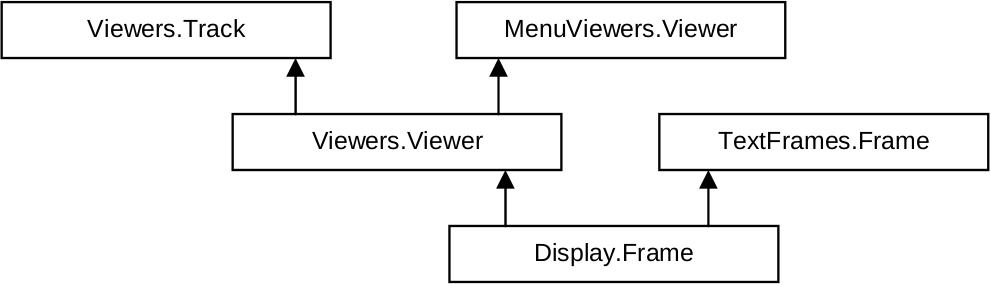
\includegraphics[width=\textwidth]{i/h}
	\caption{Extensions of type $Display.Frame$}
\end{figure}

\section{The Font Machinery}
We saw in the previous Sections that Oberon texts support attribute specifications (“looks”) for
characters. Three different attributes are supported: font, color, and vertical offset. Let us first focus
on the font attribute. A font can be regarded as a style the standard character set is designed in.
Typically, an entire text is typeset in a single style, that is, there is one font per text. However,
sometimes, an author wants to emphasize titles or words by changing the size of the font or by
varying it to bold face or italics. In special texts, special characters like mathematical symbols or
other kinds of icons may occur. In even more complex documents, mathematical or chemical
formulae might flow within the text.

This generalized view leads us to a different interpretation of the notion of font. We can regard a
font as an indexed library of (graphical) objects, mostly but not necessarily glyphs. In the case of
ordinary characters it is natural to use the ASCII-code as an index, ending up with an interpretation
of text as sequence of pairs (library, index). Note that this is a very general view indeed that, in
principle, is equivalent with defining text as sequence of arbitrary objects.

The imaging model of characters provides two levels of abstraction. On the first level, characters
are black boxes specified by a set of metric data x, y, w, h, and dx. (x, y) is a vector from the current
point of reference on the base line to the origin of the box. w and h are width and height of the box,
and dx is the distance to the point of reference of the next character on the same base line. On the
second level of abstraction, a character is defined by a digital pattern or glyph that is to be rendered
into the box. Fig \ref{fig:character} visualizes this model of characters.

The additional two character attributes color and vertical offset appear now as parameters for the
character model. The vertical offset allows translating the glyph vertically and the color attribute
specifies the foreground color of the pattern.
\begin{figure}
	\label{fig:character}
	\centering
	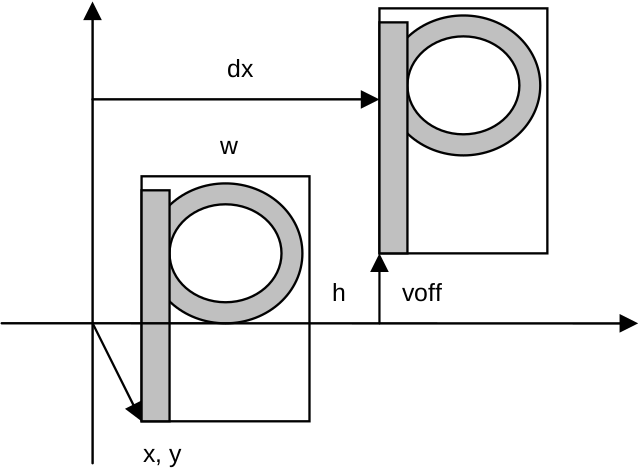
\includegraphics[width=.7\textwidth]{i/i}
	\caption{The geometric character model}
\end{figure}

Good examples of procedures operating on the first level of abstraction are procedures LocateChar
and Width that we discussed in the previous Section, as well as text formatters for a remote printer.
In contrast, procedure DisplayLine operates on the second level.

The representation of characters as digital patterns is merely the last step in a complex font design
and rendering process. At the beginning is a generic description of the shape of each character in
the form of outlines and hints. Outlines are typically composed of straight lines and spline-curves.
Hints are included to assist the digitizer in its effort to faithfully map the filled character outlines into
the device raster. For example, hinting can guarantee consistency of serif shapes and stem widths
across an entire font within a text, independent of the relative positions of the characters with
respect to the grid lines. Automatic digitization produces digital patterns of sufficiently high quality
for printing media resolutions. For screen resolutions, however, we prefer to add a hand-tuning
step. This is the reason why digital patterns are not produced "on the fly" in Oberon.

Oberon's font management is encapsulated in module Fonts, with a low-level extension into the
module Display that we already know from Chapter 4. The interface to module Fonts is very simple
and narrow:
\begin{verbatim}
MODULE Fonts;
TYPE Font = POINTER TO FontDesc;
FontDesc = RECORD
name: ARRAY 32 OF CHAR;;
height, minX, maxX, minY, maxY: INT;
next: Font
END;
VAR Default: Font;
PROC GetPat(fnt: Font; ch: CHAR; VAR dx, x, y, w, h, patadr: INT);
PROC This (name: ARRAY OF CHAR): Font;
PROC Free;
END Fonts.
\end{verbatim}

Variable name in type Font is the name of the underlying file. The variables height, minX, maxX,
minY, and maxY designate line height and summary metric data. Default is a system-wide default
font. It is installed at system loading time. GetPat delivers the geometric data for a given character
in a given font (see Figure 5.5). This is a procedure to internalize (load) a font from a file given by
its name. Free releases from storage fonts that are no longer needed.

Type Font should again be regarded as an abstract data type with two intrinsic operations This and
GetPat Thinking of the immutable nature of fonts, multiple internal copies of the same font are
certainly undesirable. Therefore, internalized fonts are cached in a private list that manifests itself in
a private field next in type FontDesc. The cache is maintained by the internalizing procedure This
according to the following scheme:
\begin{verbatim}
search font in cache;
IF found THEN return cached internalization
ELSE internalize font; cache it
END
\end{verbatim}
The implementation of type Font did not raise many challenges. One, however, is an undesirable
side-effect of caching. The problem arises if a font is used for a limited time only. Because it is
referenced by the cache it will never be collected by the system's garbage collector. Two possible
solutions offer themselves: a) provide an explicit freeing operation and b) enforce some special
handling by the garbage collector based on a concept of "weak" pointers.

We conclude this Section with a formal specification of the font file format. Note that on the one
hand, the file format is completely private to the managing Fonts module and on the other hand, it
should be ultimately stable because it is probably used for long-term backup and for wide-range
data exchange across multi-system platforms.

This is an EBNF specification of the Oberon font file format:
\begin{verbatim}
FontFile = ident header contents.
header = abstraction family variant height minX maxX minY maxY.
contents = nofRuns { beg end } { dx x y w h } { rasterByte }.
\end{verbatim}
ident, abstraction, family, and variant are one-byte values indicating file identification, abstraction
(first level without raster bytes, second level with raster bytes), font family (Times Roman, Oberon,
etc.), and variant (bold face, italics etc.). The values height, minX, maxX, minY and maxY are two
bytes long each. They define in turn line height, minimum x-coordinate (of a box), maximum xcoordinate, minimum y-coordinate, and maximum y-coordinate. All values in production contents are two bytes long. nofRuns specifies the number of runs within the ASCII-code range (intervals
occupied without gaps) and every pair [beg, end) describes one run. The tuples (dx, x, y, w, h) are
the metric data of the corresponding characters (in their ASCII-code order), and the sequence of
rasterByte gives the total of raster information.

In summary, fonts in Oberon are indexed libraries of objects. The objects are descriptions of
character images in two levels of abstraction: As metric data of black boxes and as binary patterns
(glyphs). Type Font is an abstract data type with intrinsic operations to internalize and to get
character object data. Internalized fonts are cached in a private list.

\section{The Edit toolbox}
We have seen that every text frame integrates an interactive text editor that we can regard as an
interpreter of a set of built-in commands (intrinsic commands). Of course, we would like to be able
to extend this set by custom editing commands (extrinsic commands). Adding additional editing
commands was indeed a worthwhile stress test for the underlying texts API. Module Edit is the
result of this effort. It is a toolbox of consisting of some standard extrinsic editing commands.
\begin{verbatim}
DEFINITION Edit;
PROC Open; (*text viewer*)
PROC Show; (*text*)
PROC Locate; (*position*)
PROC Search; (*pattern*)
PROC Store; (*text*)
PROC Recall; (*deleted text*)
PROC CopyFont;
PROC ChangeFont;
PROC ChangeColor;
PROC ChangeOffset;
END Edit.
\end{verbatim}

The first group of commands in Edit is used to display, locate, and store texts or parts of texts. In
turn they open a text file and display it, open a program text and show the declaration of a given
object, locate a given position in a displayed text (main application: locating an error found by the
compiler), search a pattern, and store the current state of a displayed text. Commands in the next
group are related with editing. They allow restoring of the previously deleted part of text, copying a
font attribute to the current text selection, and change attributes of the current text selection. Note
that the commands CopyFont, ChangeFont, ChangeColor, and ChangeOffset are extrinsic
variations of the intrinsic copy-look operation. The implementations of the toolbox commands are
given in the Appendix.

\section*{References}
\begin{description}
	\item[Gutknecht] J. Gutknecht, "Concept of the Text Editor Lara", Communications of the ACM, Sept. 1985, Vol.28, No.9.
	\item[Teitelman] W. Teitelman, "A tour through Cedar", IEEE Software, 1, (2), 44-73 (1984).
\end{description}
